\documentclass[a4paper,11pt]{article}
\usepackage{amsmath,amsthm,amsfonts,amssymb,amscd,amstext,vmargin,graphics,graphicx,tabularx,multicol} 
\usepackage[francais]{babel}
\usepackage[utf8]{inputenc}  
\usepackage[T1]{fontenc} 
\usepackage{pstricks-add,tikz,tkz-tab,variations}
\usepackage[autolanguage,np]{numprint} 

\setmarginsrb{1.5cm}{0.5cm}{1cm}{0.5cm}{0cm}{0cm}{0cm}{0cm} %Gauche, haut, droite, haut
\newcounter{numexo}
\newcommand{\exo}[1]{\stepcounter{numexo}\noindent{\bf \underline{Exercice~\thenumexo}}}
\reversemarginpar


\newcounter{enumtabi}
\newcounter{enumtaba}
\newcommand{\q}{\stepcounter{enumtabi} \theenumtabi.  }
\newcommand{\qa}{\stepcounter{enumtaba} (\alph{enumtaba}) }
\newcommand{\initq}{\setcounter{enumtabi}{0}}
\newcommand{\initqa}{\setcounter{enumtaba}{0}}

\newcommand{\be}{\begin{enumerate}}
\newcommand{\ee}{\end{enumerate}}
\newcommand{\bi}{\begin{itemize}}
\newcommand{\ei}{\end{itemize}}
\newcommand{\bp}{\begin{pspicture*}}
\newcommand{\ep}{\end{pspicture*}}
\newcommand{\bt}{\begin{tabular}}
\newcommand{\et}{\end{tabular}}
\renewcommand{\tabularxcolumn}[1]{>{\centering}m{#1}} %(colonne m{} centrée, au lieu de p par défault) 
\newcommand{\tnl}{\tabularnewline}

\newcommand{\bmul}[1]{\begin{multicols}{#1}}
\newcommand{\emul}{\end{multicols}}

\newcommand{\trait}{\noindent \rule{\linewidth}{0.2mm}}
\newcommand{\hs}[1]{\hspace{#1}}
\newcommand{\vs}[1]{\vspace{#1}}

\newcommand{\N}{\mathbb{N}}
\newcommand{\Z}{\mathbb{Z}}
\newcommand{\R}{\mathbb{R}}
\newcommand{\C}{\mathbb{C}}
\newcommand{\Dcal}{\mathcal{D}}
\newcommand{\Ccal}{\mathcal{C}}
\newcommand{\mc}{\mathcal}

\newcommand{\vect}[1]{\overrightarrow{#1}}
\newcommand{\ds}{\displaystyle}
\newcommand{\eq}{\quad \Leftrightarrow \quad}
\newcommand{\vecti}{\vec{\imath}}
\newcommand{\vectj}{\vec{\jmath}}
\newcommand{\Oij}{(O;\vec{\imath}, \vec{\jmath})}
\newcommand{\OIJ}{(O;I,J)}




\newcommand{\reponse}[1][1]{%
\multido{}{#1}{\makebox[\linewidth]{\rule[0pt]{0pt}{20pt}\dotfill}
}}

\newcommand{\titre}[5] 
% #1: titre #2: haut gauche #3: bas gauche #4: haut droite #5: bas droite
{
\noindent #2 \hfill #4 \\
#3 \hfill #5

\vspace{-1.6cm}

\begin{center}\rule{6cm}{0.5mm}\end{center}
\vspace{0.2cm}
\begin{center}{\large{\textbf{#1}}}\end{center}
\begin{center}\rule{6cm}{0.5mm}\end{center}
}



\begin{document}
\pagestyle{empty}
\titre{Chapitre 10 : Périmètre et aire}{}{}{}{}

\vspace*{1cm}

\begin{center}
{\Large \textbf{Niveau 1 :}}
\end{center}

\vspace*{1cm}

$\rightarrow$ \textbf{Conversion des longueurs (m)}\\

\vspace*{0.5cm}

\exo \\  A l'aide du tableau de conversion ci-dessous,  exprimer les longueurs dans l'unité demandée.\\

\begin{tabular}{|c|c|c|c|c|c|c|}
\hline 
km & hm & dam & m & dm & cm & mm \\ 
\hline 
\end{tabular} 

\vspace{0.75cm}


\initqa \qa 1 cm = . . . . mm\\

\qa 1 km = . . . . m\\

\qa 1 dam = . . . . dm\\

\qa 1 hm = . . . . cm\\

\qa 1 m = . . . . cm\\

\qa 1 dm = . . . . mm\\


\exo \\  

\vspace{0.75cm}

\begin{tabular}{|c|c|c|c|c|c|c|}
\hline 
km & hm & dam & m & dm & cm & mm \\ 
\hline 
\end{tabular} 

\vspace{0.75cm}

Sachant que 1 m = 100 cm. Convertir les longueurs ci-dessous en cm.\\

Un exemple pour vous aider,  4 m =  $4 \times$ 100 cm =  400 cm.\\


\initqa \qa 8 m = . . . . cm\\

\qa 1 209 m = . . . . cm\\

\qa 935 m = . . . . cm\\

\qa 74 m= . . . . cm\\


\exo \\ Compléter par les unités de longueur qui conviennent.\\

\initqa \qa 23,047 m = 2 . . + 3 . . + 4 . . + 7 . . \\

\qa  3,520 km = 3 . . + 5 . . + 2 . .  \\

\qa  51,04 m = 5 . . + 1 . . + 4 . . \\

\qa 0,765 km = 7 . . + 6 . . + 5 . .  \\


\vspace*{1cm}

$\rightarrow$ \textbf{Conversion : unités d'aire ($m^{2}$)}\\

\vspace*{0.5cm}

\exo \\  A l'aide du tableau de conversion ci-dessous,  exprimer les aires dans l'unité demandée.\\

\vspace*{0.75cm}

\begin{tabular}{|p{0.5cm}|p{0.5cm}|p{0.5cm}|p{0.5cm}|p{0.5cm}|p{0.5cm}|p{0.5cm}|p{0.5cm}|p{0.5cm}|p{0.5cm}|p{0.5cm}|p{0.5cm}|p{0.5cm}|p{0.5cm}|}
\hline 
\multicolumn{2}{|c|}{$km^{2}$} & \multicolumn{2}{|c|}{$hm^{2}$} & \multicolumn{2}{|c|}{$dam^{2}$} & \multicolumn{2}{|c|}{$m^{2}$} & \multicolumn{2}{|c|}{$dm^{2}$} & \multicolumn{2}{|c|}{$cm^{2}$} & \multicolumn{2}{|c|}{$mm^{2}$} \\ 
\hline 
 &  &  & ha &  & a &  & ca &  &  &  &  &  &  \\ 
\hline 
\end{tabular} 

\vspace*{0.75cm}


\initqa \qa 3  $m^{2}$ = . . . . . $dm^{2}$ = . . . . . $cm^{2}$\\

 \qa 3  $m^{2}$ = . . . . . $dam^{2}$ = . . . . . $hm^{2}$\\
 
 
 
 \exo \\

\vspace*{0.75cm}

\begin{tabular}{|p{0.5cm}|p{0.5cm}|p{0.5cm}|p{0.5cm}|p{0.5cm}|p{0.5cm}|p{0.5cm}|p{0.5cm}|p{0.5cm}|p{0.5cm}|p{0.5cm}|p{0.5cm}|p{0.5cm}|p{0.5cm}|}
\hline 
\multicolumn{2}{|c|}{$km^{2}$} & \multicolumn{2}{|c|}{$hm^{2}$} & \multicolumn{2}{|c|}{$dam^{2}$} & \multicolumn{2}{|c|}{$m^{2}$} & \multicolumn{2}{|c|}{$dm^{2}$} & \multicolumn{2}{|c|}{$cm^{2}$} & \multicolumn{2}{|c|}{$mm^{2}$} \\ 
\hline 
 &  &  & ha &  & a &  & ca &  &  &  &  &  &  \\ 
\hline 
\end{tabular} 

\vspace*{0.75cm}
 
 
 Sachant que 1 $dam^{2}$ = 100 $m^{2}$. Convertir les aires ci-dessous en $m^{2}$.\\

Un exemple pour vous aider,  7 $dam^{2}$ =  $7 \times$ 100 $m^{2}$ =  700 $m^{2}$.\\


\initqa \qa 11 $dam^{2}$ = . . . . . . . . . $m^{2}$\\

\qa 7 560 $dam^{2}$ = . . . . . . . . . $m^{2}$\\

\qa 5 $dam^{2}$ = . . . . . . . . . $m^{2}$\\

\qa 143 $dam^{2}$ = . . . . . . . . . $m^{2}$\\


\vspace*{0.5cm}


\vspace*{1cm}

$\rightarrow$ \textbf{Périmètre d'un polygone / cercle}\\

\vspace*{0.5cm}

\exo \\ Compléter la définition du périmètre d'une figure.\\

Le mot périmètre provient du grec ancien \textit{perimetros} qui signifie "mesure du tour", c'est donc la longueur du . . . . . . . . d'une figure.\\

\exo \\ Observer   attentivement   l'unité   de   longueur (1 u.l.) puis déterminer le périmètre, en unités de longueur, de chaque figure.\\


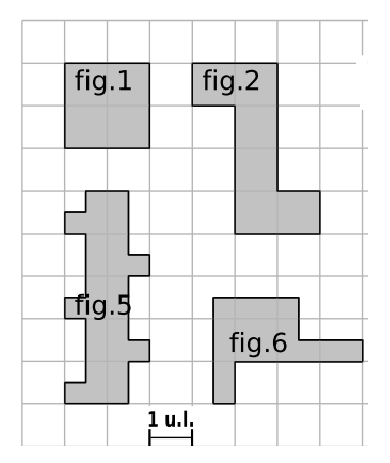
\includegraphics[scale=0.8]{figperimetrecompte.eps} \\

figure 1 : . . . . \\

figure 2 : . . . . \\

figure 5 : . . . . \\

figure 6 : . . . . \\


\exo \\ Compléter la formule pour calculer le périmètre d'un carré de côté \textit{c}.\\

$P=....................$\\


\exo \\ Compléter la formule pour calculer le périmètre d'un rectangle de longueur \textit{L} et de largeur \textit{l}.\\

$P=....................$\\


\vspace*{1cm}

$\rightarrow$ \textbf{Périmètre de figures complexes}\\

\vspace*{0.5cm}



\exo \\ Calculer le périmètre de la figure ci-dessous, après avoir complété sa description.\\

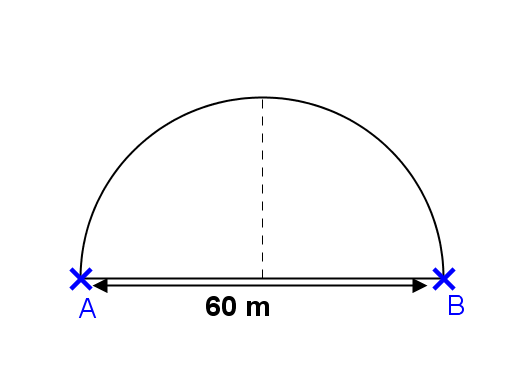
\includegraphics[scale=1]{complexe1.eps} 

\textbf{Description :} Cette figure est composée de . . . quart(s) de cercle et de . . . . segment(s).\\

Formule(s) utilisée(s) : . . . . . . . . . . . . . . .\\

Calculs :\\
\reponse[2]\\

Réponse : . . . . . . . . . . . . . . .\\




\exo \\ Calculer le périmètre de la figure ci-dessous, après avoir complété sa description.\\

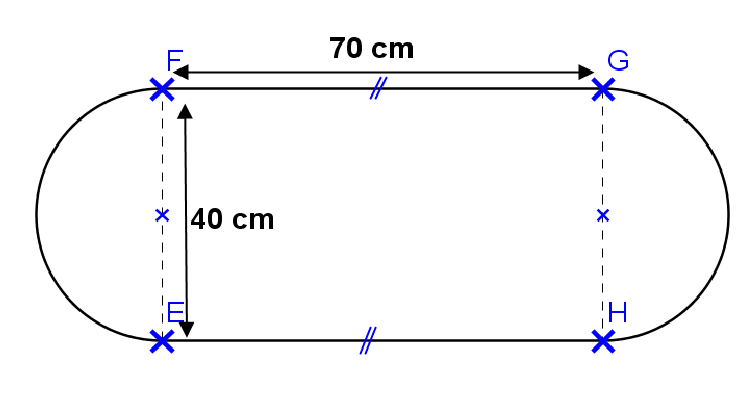
\includegraphics[scale=1]{complexe2.eps} 

\textbf{Description :} Cette figure est composée de . . . demi(s)-cercle de même rayon et de . . . . segment(s).\\

Formule(s) utilisée(s) : . . . . . . . . . . . . . . .\\

Calculs :\\
\reponse[2]\\

Réponse : . . . . . . . . . . . . . . .\\



\vspace*{1cm}

$\rightarrow$ \textbf{Aire de figures usuelles}\\

\vspace*{0.5cm}


\exo \\ Compléter la formule pour calculer l'aire d'un carré de côté \textit{c}.\\

$A=....................$\\


\exo \\ Compléter la formule pour calculer l'aire d'un rectangle de longueur \textit{L} et de largeur \textit{l}.\\

$A=....................$\\


\exo \\ Dans cet exercice, une unité d'aire est représentée par un carreau. Indiquer l'aire des figures suivantes.\\


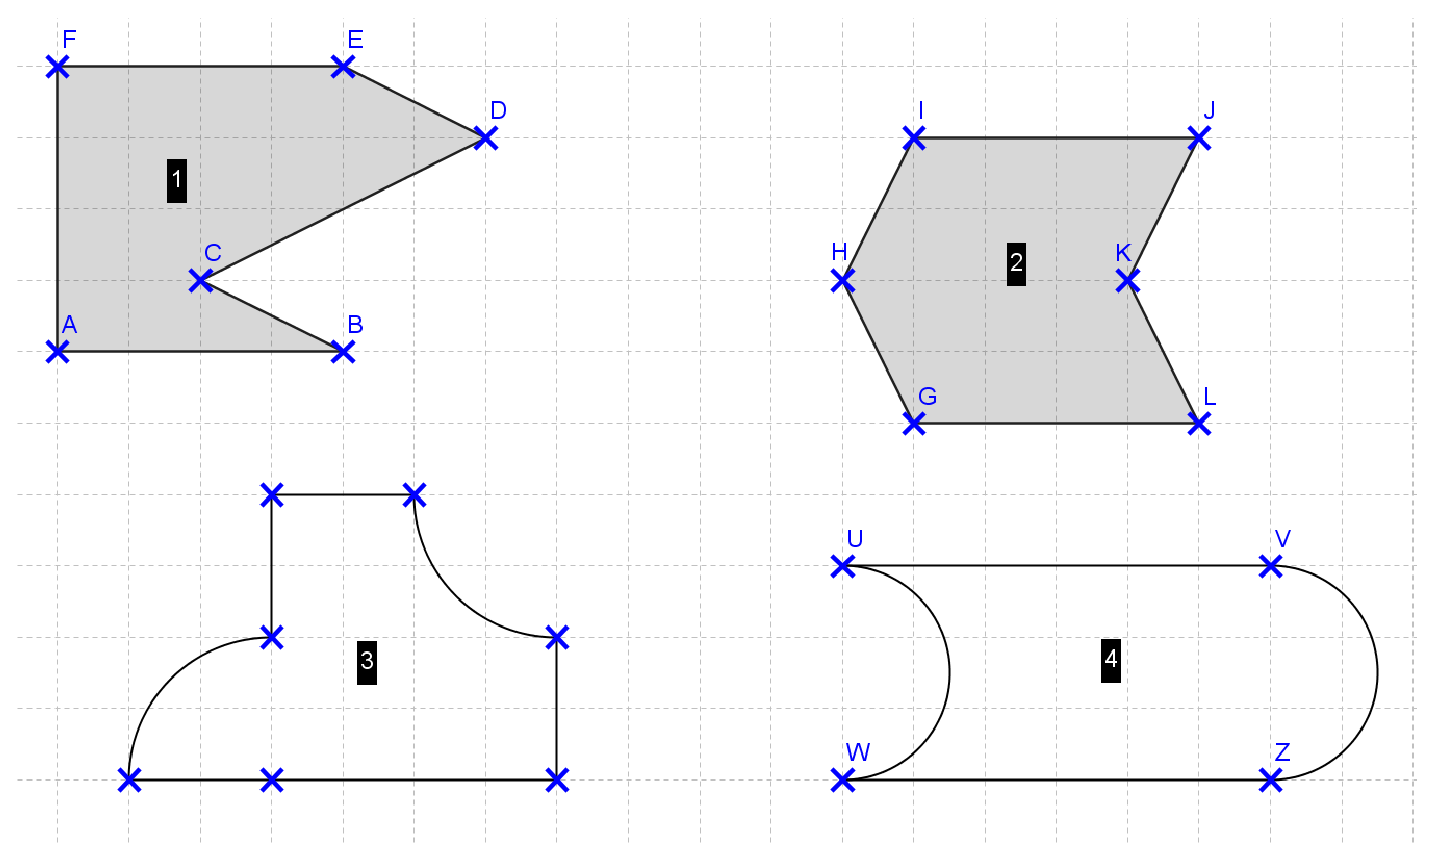
\includegraphics[scale=0.8]{aire1.eps} \\

figure 1 : . . . . \\

figure 2 : . . . . \\

figure 3 : . . . . \\

figure 4 : . . . . \\


\vspace*{1cm}

$\rightarrow$ \textbf{Aire de figures complexes}\\

\vspace*{0.5cm}






\exo \\ Calculer l'aire de la figure ci-dessous.\\

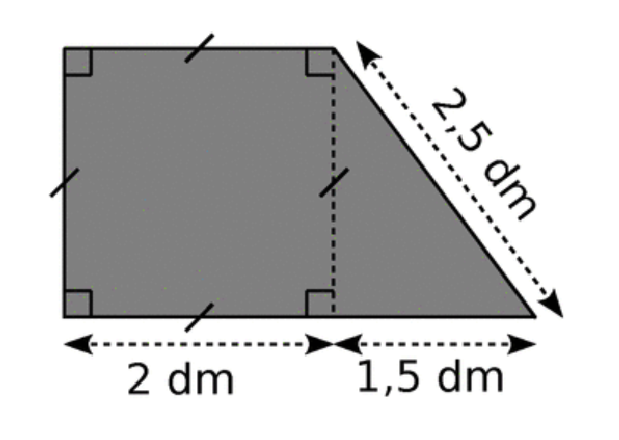
\includegraphics[scale=1]{airecomplexe11.eps} \\

Formules utilisées : . . . . . . . . . . . . . . .\\

Calculs :\\
\reponse[3]\\


Réponse : . . . . . . . . . . . . . . .\\






	

\begin{center}
{\Large \textbf{Niveau 2 :}}
\end{center}

\vspace*{1cm}

$\rightarrow$ \textbf{Conversion des longueurs (m)}\\

\vspace*{0.5cm}





\exo \\  

\vspace{0.75cm}

\begin{tabular}{|c|c|c|c|c|c|c|}
\hline 
km & hm & dam & m & dm & cm & mm \\ 
\hline 
\end{tabular} 

\vspace{0.75cm}

Sachant que 1 km = 1 000 m. Convertir les longueurs ci-dessous en m.\\

Un exemple pour vous aider,  14 km =  $14 \times$ 1 000 m = 14 000 m.\\


\initqa \qa 8 km = . . . . m\\

\qa 54 km = . . . . m\\

\qa 1 325 km = . . . . m\\

\qa 107 km = . . . . m\\



\exo \\  A l'aide du tableau de conversion ci-dessous,  exprimer les longueurs dans l'unité demandée.\\

\begin{tabular}{|c|c|c|c|c|c|c|}
\hline 
km & hm & dam & m & dm & cm & mm \\ 
\hline 
\end{tabular} 

\vspace{0.75cm}

\initqa \qa 58 dam = . . . . m\\

\qa 12 hm = . . . . cm\\

\qa 5 km = . . . . dam\\

\qa 702 m = . . . . mm\\

\qa 98 dm = . . . . mm\\

\qa 435 dam = . . . . dm\\



\vspace*{0.5cm}



\vspace*{1cm}

$\rightarrow$ \textbf{Conversion : unités d'aire ($m^{2}$)}\\

\vspace*{0.5cm}




 \exo \\

\vspace*{0.75cm}

\begin{tabular}{|p{0.5cm}|p{0.5cm}|p{0.5cm}|p{0.5cm}|p{0.5cm}|p{0.5cm}|p{0.5cm}|p{0.5cm}|p{0.5cm}|p{0.5cm}|p{0.5cm}|p{0.5cm}|p{0.5cm}|p{0.5cm}|}
\hline 
\multicolumn{2}{|c|}{$km^{2}$} & \multicolumn{2}{|c|}{$hm^{2}$} & \multicolumn{2}{|c|}{$dam^{2}$} & \multicolumn{2}{|c|}{$m^{2}$} & \multicolumn{2}{|c|}{$dm^{2}$} & \multicolumn{2}{|c|}{$cm^{2}$} & \multicolumn{2}{|c|}{$mm^{2}$} \\ 
\hline 
 &  &  & ha &  & a &  & ca &  &  &  &  &  &  \\ 
\hline 
\end{tabular} 

\vspace*{0.75cm}
 
 
 Sachant que 1 $m^{2}$ = 10 000 $cm^{2}$. Convertir les aires ci-dessous en $cm^{2}$.\\

Un exemple pour vous aider,  7 $m^{2}$ =  $7 \times$ 10 000 $cm^{2}$ =  70 000 $cm^{2}$.\\


\initqa \qa 106 $m^{2}$ = . . . . . . . . . $cm^{2}$\\

\qa 23 $m^{2}$ = . . . . . . . . . $cm^{2}$\\

\qa 1 074 $m^{2}$ = . . . . . . . . . $cm^{2}$\\

\qa 9 $m^{2}$ = . . . . . . . . . $cm^{2}$\\


\vspace*{1cm}

$\rightarrow$ \textbf{Périmètre d'un polygone / cercle}\\

\vspace*{0.5cm}




\exo \\ Calculer le périmètre du carré ABCD ci-dessous.\\

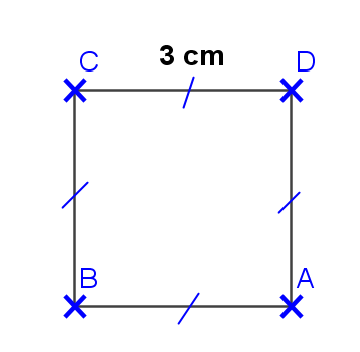
\includegraphics[scale=1]{perimetre1.eps} \\

Formule : . . . . . . . . . . . . . . .\\

Calculs : . . . . . . . . . . . . . . .\\

Réponse : . . . . . . . . . . . . . . .\\


\exo \\ Calculer le périmètre du rectangle EFGH ci-dessous.\\

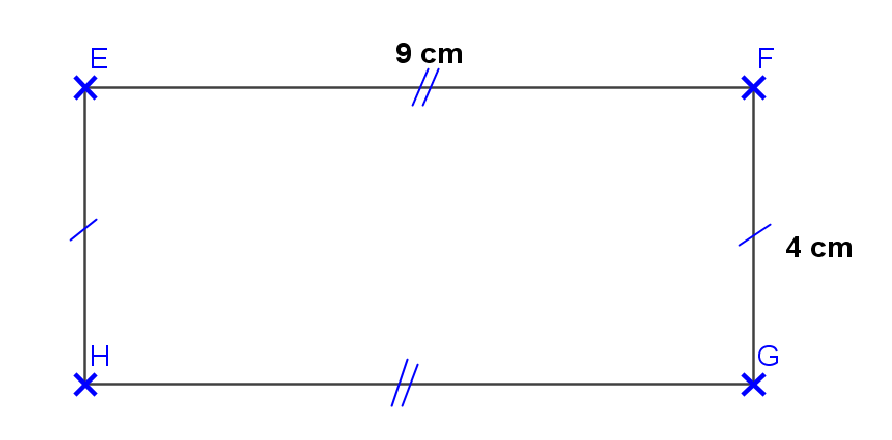
\includegraphics[scale=1]{perimetre2.eps} \\


Formule : . . . . . . . . . . . . . . .\\

Calculs : . . . . . . . . . . . . . . .\\

Réponse : . . . . . . . . . . . . . . .\\



\exo \\ Calculer le périmètre d'un rectangle MLKJ tel que ML = 9 m et LK = 5,3 m. \\

Formule : . . . . . . . . . . . . . . .\\

Calculs : . . . . . . . . . . . . . . .\\

Réponse : . . . . . . . . . . . . . . .\\




\exo \\ Calculer le périmètre d'un carré OLKI tel que OL = 7,5 dm.  \\



Formule : . . . . . . . . . . . . . . .\\

Calculs : . . . . . . . . . . . . . . .\\

Réponse : . . . . . . . . . . . . . . .\\


\vspace*{1cm}

$\rightarrow$ \textbf{Périmètre de figures complexes}\\

\vspace*{0.5cm}




\exo \\ Calculer le périmètre de la figure ci-dessous, après avoir complété sa description.\\

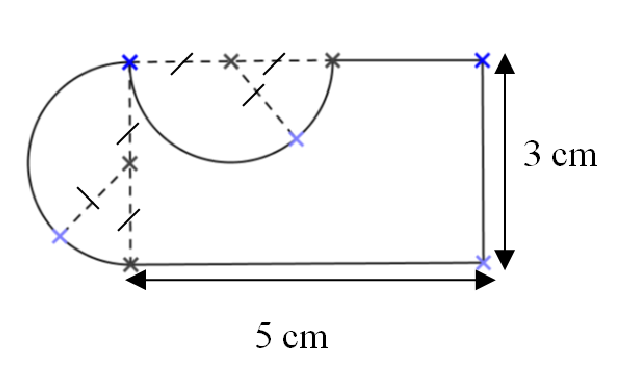
\includegraphics[scale=1]{complexe3.eps} 

\textbf{Description :} Cette figure est composée de . . . demi(s)-cercle de même rayon et de . . . . segment(s).\\

Formule(s) utilisée(s) : . . . . . . . . . . . . . . .\\

Calculs :\\
\reponse[2]\\

Réponse : . . . . . . . . . . . . . . .\\





\vspace*{1cm}

$\rightarrow$ \textbf{Aire de figures usuelles}\\

\vspace*{0.5cm}





\exo \\ Calculer l'aire du carré ABCD ci-dessous.\\

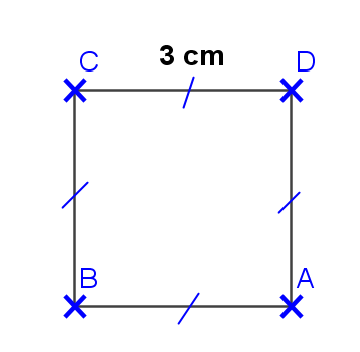
\includegraphics[scale=1]{perimetre1.eps} \\

Formule : . . . . . . . . . . . . . . .\\

Calculs : . . . . . . . . . . . . . . .\\

Réponse : . . . . . . . . . . . . . . .\\


\exo \\ Calculer l'aire du rectangle EFGH ci-dessous.\\

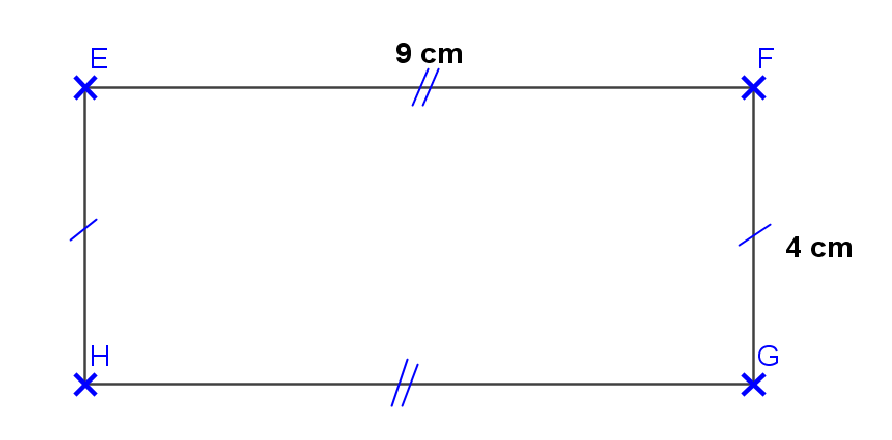
\includegraphics[scale=1]{perimetre2.eps} \\


Formule : . . . . . . . . . . . . . . .\\

Calculs : . . . . . . . . . . . . . . .\\

Réponse : . . . . . . . . . . . . . . .\\



\exo \\ Calculer l'aire d'un rectangle MLKJ tel que ML = 10 m et LK = 14,6 m. \\

Formule : . . . . . . . . . . . . . . .\\

Calculs : . . . . . . . . . . . . . . .\\

Réponse : . . . . . . . . . . . . . . .\\




\exo \\ Calculer l'aire d'un carré OLKI tel que OL = 50 dm.  \\



Formule : . . . . . . . . . . . . . . .\\

Calculs : . . . . . . . . . . . . . . .\\

Réponse : . . . . . . . . . . . . . . .\\






\vspace*{1cm}

$\rightarrow$ \textbf{Aire de figures complexes}\\

\vspace*{0.5cm}


\exo \\ Calculer l'aire du polygone ABCD suivant.\\

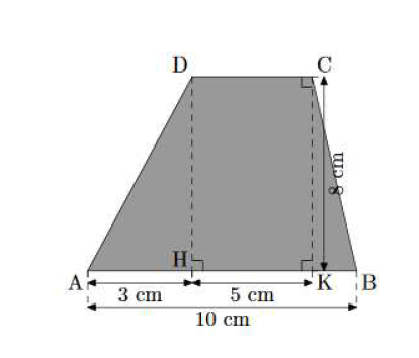
\includegraphics[scale=1]{airecomplexe4.eps} \\

Formules utilisées : . . . . . . . . . . . . . . .\\

Calculs :\\
\reponse[3]\\


Réponse : . . . . . . . . . . . . . . .\\


\exo \\ Calculer l'aire de la surface ABCDEFG ci-dessous.\\

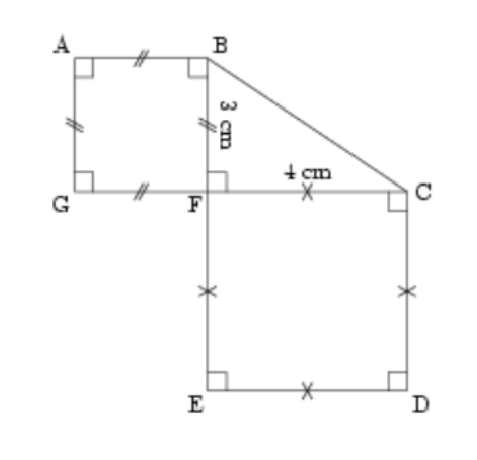
\includegraphics[scale=1]{airecomplexe2.eps} \\



Formules utilisées : . . . . . . . . . . . . . . .\\

Calculs :\\
\reponse[3]\\

Réponse : . . . . . . . . . . . . . . .\\







\begin{center}
{\Large \textbf{Niveau 3 :}}
\end{center}

\vspace*{1cm}

$\rightarrow$ \textbf{Conversion des longueurs (m)}\\

\vspace*{0.5cm}


\exo \\  A l'aide du tableau de conversion ci-dessous,  exprimer les longueurs dans l'unité demandée.\\

\begin{tabular}{|c|c|c|c|c|c|c|}
\hline 
km & hm & dam & m & dm & cm & mm \\ 
\hline 
\end{tabular} 

\vspace{0.75cm}

\initqa \qa 103 cm = . . . . m\\

\qa 10 326 dm = . . . . hm\\

\qa 581 407 mm = . . . . dam\\

\qa 15 dam = . . . . km\\

\qa 9 mm = . . . . m\\

\qa 22 m = . . . . km\\




\exo \\  

\vspace{0.75cm}

\begin{tabular}{|c|c|c|c|c|c|c|}
\hline 
km & hm & dam & m & dm & cm & mm \\ 
\hline 
\end{tabular} 

\vspace{0.75cm}

Sachant que 1 m = 0,01 hm. Convertir les longueurs ci-dessous en hm.\\

Un exemple pour vous aider :  7 126 m =  7 126 $\times$ 0,01 hm = 71,26 hm.\\


\initqa \qa 6 m = . . . . hm\\

\qa 11 529 m = . . . . hm\\

\qa 93 m = . . . . hm\\

\qa 402 537 km = . . . . hm\\


\vspace*{1cm}

$\rightarrow$ \textbf{Conversion : unités d'aire ($m^{2}$)}\\

\vspace*{0.5cm}




\exo \\  A l'aide du tableau de conversion ci-dessous,  exprimer les aires dans l'unité demandée.\\

\vspace*{0.75cm}

\begin{tabular}{|p{0.5cm}|p{0.5cm}|p{0.5cm}|p{0.5cm}|p{0.5cm}|p{0.5cm}|p{0.5cm}|p{0.5cm}|p{0.5cm}|p{0.5cm}|p{0.5cm}|p{0.5cm}|p{0.5cm}|p{0.5cm}|}
\hline 
\multicolumn{2}{|c|}{$km^{2}$} & \multicolumn{2}{|c|}{$hm^{2}$} & \multicolumn{2}{|c|}{$dam^{2}$} & \multicolumn{2}{|c|}{$m^{2}$} & \multicolumn{2}{|c|}{$dm^{2}$} & \multicolumn{2}{|c|}{$cm^{2}$} & \multicolumn{2}{|c|}{$mm^{2}$} \\ 
\hline 
 &  &  & ha &  & a &  & ca &  &  &  &  &  &  \\ 
\hline 
\end{tabular} 

\vspace*{0.75cm}



\initqa \qa 1,3 $mm^{2}$ = . . . . . . . . . . $cm^{2}$\\

\qa 0,74 $dm^{2}$ = . . . . . . . . . . $cm^{2}$\\

\qa 568 $cm^{2}$ = . . . . . . . . . . $m^{2}$\\

\qa 2 $hm^{2}$ = . . . . . . . . . . $km^{2}$\\

\qa 9,7 $km^{2}$ = . . . . . . . . . . $m^{2}$\\









\exo \\  A l'aide du tableau de conversion ci-dessous,  exprimer toutes les aires données en $cm^{2}$.\\

\vspace*{0.75cm}

\begin{tabular}{|p{0.5cm}|p{0.5cm}|p{0.5cm}|p{0.5cm}|p{0.5cm}|p{0.5cm}|p{0.5cm}|p{0.5cm}|p{0.5cm}|p{0.5cm}|p{0.5cm}|p{0.5cm}|p{0.5cm}|p{0.5cm}|}
\hline 
\multicolumn{2}{|c|}{$km^{2}$} & \multicolumn{2}{|c|}{$hm^{2}$} & \multicolumn{2}{|c|}{$dam^{2}$} & \multicolumn{2}{|c|}{$m^{2}$} & \multicolumn{2}{|c|}{$dm^{2}$} & \multicolumn{2}{|c|}{$cm^{2}$} & \multicolumn{2}{|c|}{$mm^{2}$} \\ 
\hline 
 &  &  & ha &  & a &  & ca &  &  &  &  &  &  \\ 
\hline 
\end{tabular} 

\vspace*{0.75cm}



\initqa \qa 32,7 $m^{2}$ = . . . . . . . . . . $cm^{2}$\\

\qa 0,04 $dm^{2}$ = . . . . . . . . . . $cm^{2}$\\

\qa 6 200 $mm^{2}$ = . . . . . . . . . . $cm^{2}$\\

\qa 2,19 $dam^{2}$ = . . . . . . . . . . $cm^{2}$\\





\exo \\ \exo \\  A l'aide du tableau de conversion ci-dessous,  exprimer les aires données dans l'unité demandée.\\

\vspace*{0.75cm}

\begin{tabular}{|p{0.5cm}|p{0.5cm}|p{0.5cm}|p{0.5cm}|p{0.5cm}|p{0.5cm}|p{0.5cm}|p{0.5cm}|p{0.5cm}|p{0.5cm}|p{0.5cm}|p{0.5cm}|p{0.5cm}|p{0.5cm}|}
\hline 
\multicolumn{2}{|c|}{$km^{2}$} & \multicolumn{2}{|c|}{$hm^{2}$} & \multicolumn{2}{|c|}{$dam^{2}$} & \multicolumn{2}{|c|}{$m^{2}$} & \multicolumn{2}{|c|}{$dm^{2}$} & \multicolumn{2}{|c|}{$cm^{2}$} & \multicolumn{2}{|c|}{$mm^{2}$} \\ 
\hline 
 &  &  & ha &  & a &  & ca &  &  &  &  &  &  \\ 
\hline 
\end{tabular} 

\vspace*{0.75cm}


\initqa \qa 75 $dam^{2}$ = . . . . . . a\\

 \qa 390 $m^{2}$ = . . . . . . a\\
 
  \qa 6,7 $hm^{2}$ = . . . . . . a\\
  
   \qa 72 ha = . . . . . . a\\
   
   \qa 9 $km^{2}$ = . . . . . . ha\\
   
   \qa 10,5 $dam^{2}$ = . . . . . . ha\\



\vspace*{1cm}

$\rightarrow$ \textbf{Périmètre d'un polygone / cercle}\\

\vspace*{0.5cm}


\exo \\  Calculer le périmètre du triangle RST quelconque ci-dessous.\\

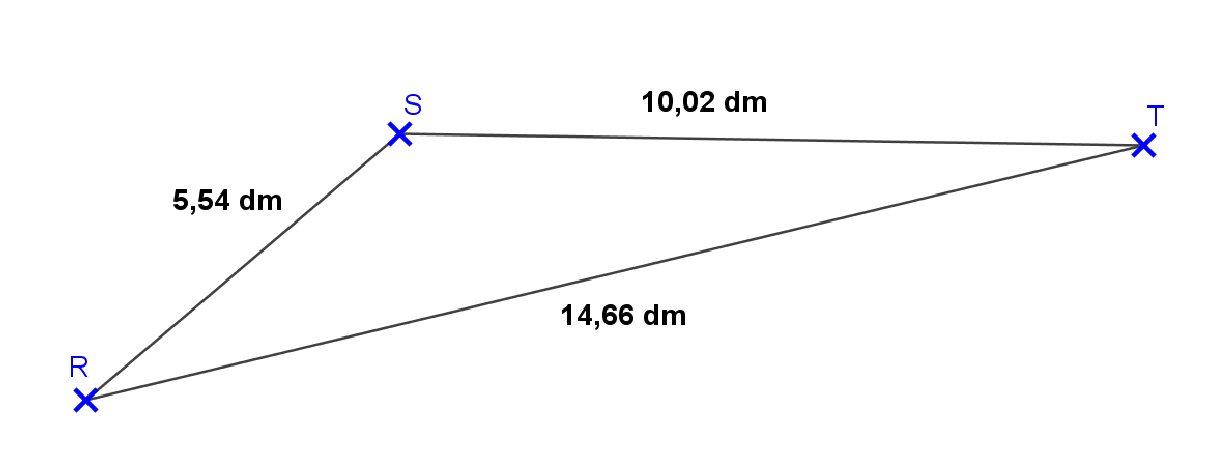
\includegraphics[scale=0.9]{perimetre6.eps} \\



Calculs : . . . . . . . . . . . . . . .\\

Réponse : . . . . . . . . . . . . . . .\\

\exo \\  Calculer le périmètre du triangle IJK isocèle en K ci-dessous.\\

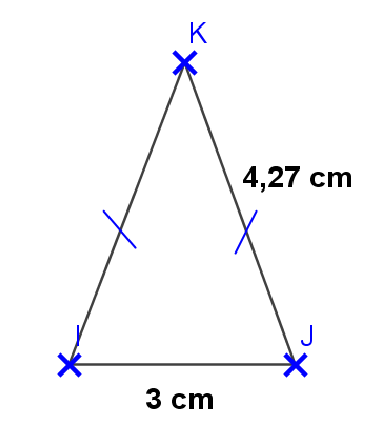
\includegraphics[scale=1]{perimetre3.eps} \\



Calculs : . . . . . . . . . . . . . . .\\

Réponse : . . . . . . . . . . . . . . .\\


\exo \\  Calculer le périmètre du triangle LMN rectangle en M ci-dessous.\\

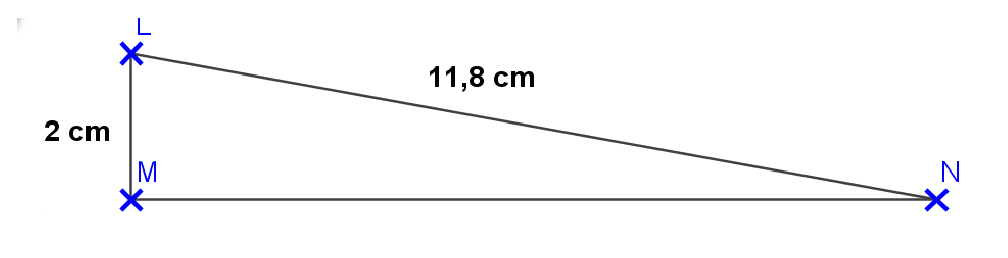
\includegraphics[scale=1]{perimetre4.eps} \\



Calculs : . . . . . . . . . . . . . . .\\

Réponse : . . . . . . . . . . . . . . .\\

\exo \\  Calculer le périmètre du triangle OPQ équilatéral ci-dessous.\\

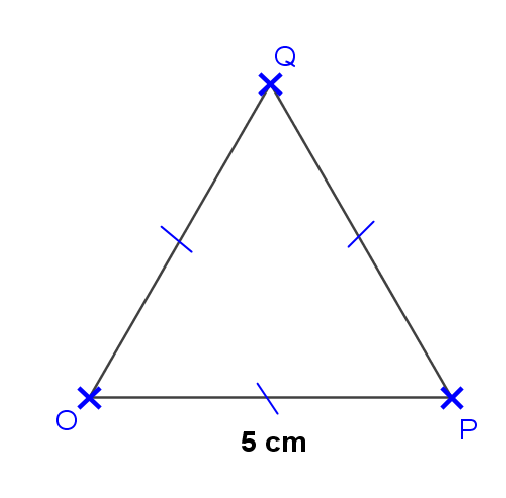
\includegraphics[scale=1]{perimetre5.eps} \\



Calculs : . . . . . . . . . . . . . . .\\

Réponse : . . . . . . . . . . . . . . .\\


\exo \\  Calculer le périmètre du polygone ci-dessous, les longueurs sur la figure sont en millimètres.\\

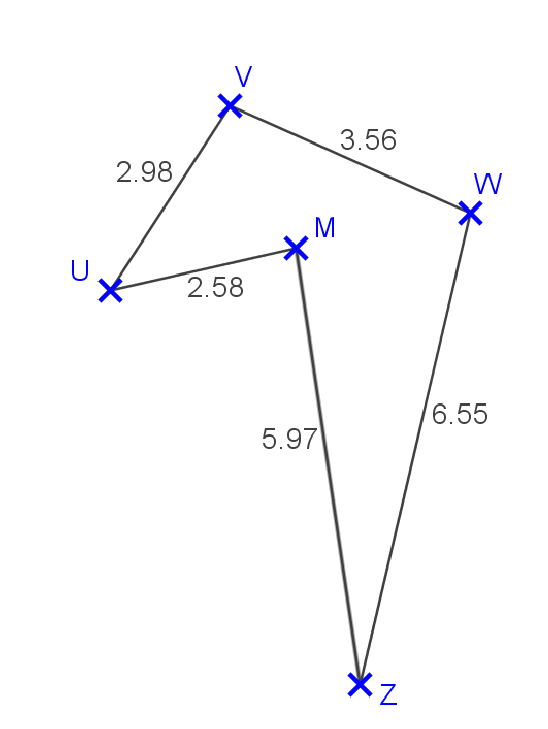
\includegraphics[scale=0.9]{perimetre7.eps} \\



Calculs : . . . . . . . . . . . . . . .\\

Réponse : . . . . . . . . . . . . . . .\\


\exo \\  Calculer le périmètre de l'octogone régulier ci-dessous.\\

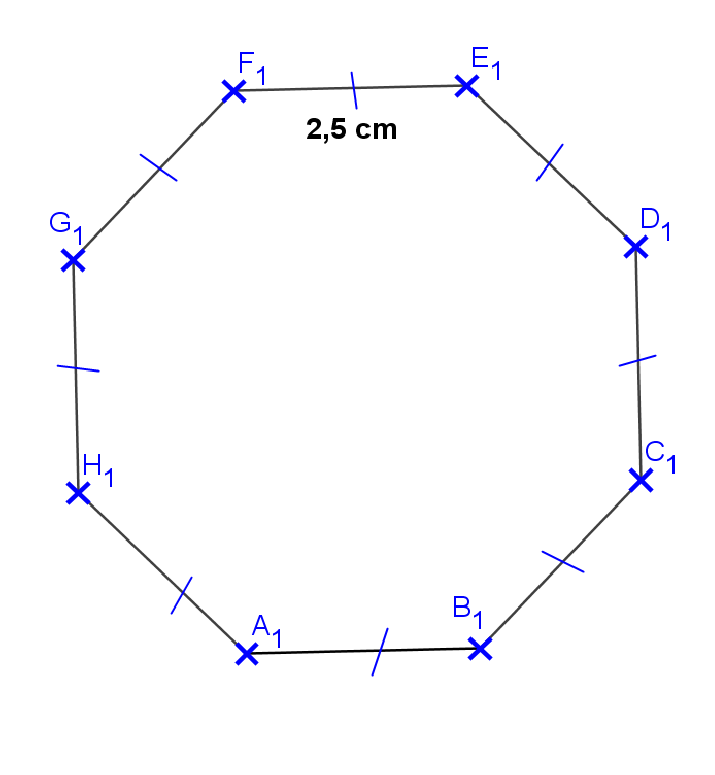
\includegraphics[scale=0.9]{perimetre8.eps} \\



Calculs : . . . . . . . . . . . . . . .\\

Réponse : . . . . . . . . . . . . . . .\\


\vspace*{1cm}

$\rightarrow$ \textbf{Périmètre de figures complexes}\\

\vspace*{0.5cm}




\exo \\ Calculer le périmètre de la figure ci-dessous, après avoir complété sa description.\\

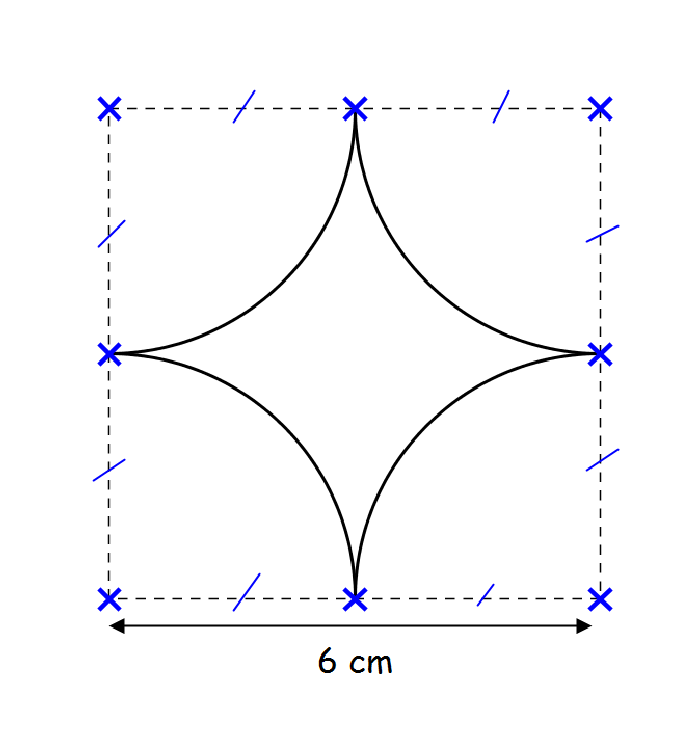
\includegraphics[scale=1]{complexe8.eps} 

\textbf{Description :} Cette figure est composée de . . .  quart(s) de cercle de même rayon et de . . . . segment(s).\\

Formule(s) utilisée(s) : . . . . . . . . . . . . . . .\\

Calculs :\\
\reponse[2]\\

Réponse : . . . . . . . . . . . . . . .\\




\exo \\ Calculer le périmètre de la figure ci-dessous, après avoir complété sa description.\\

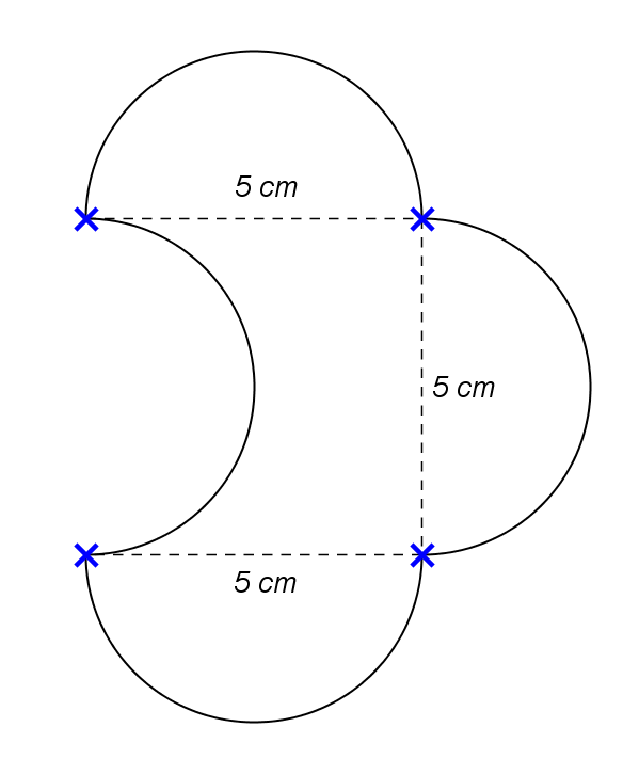
\includegraphics[scale=1]{complexe9.eps} 

\textbf{Description :} Cette figure est composée de . . .  demi(s)-cercle de même rayon et de . . . . segment(s).\\

Formule(s) utilisée(s) : . . . . . . . . . . . . . . .\\

Calculs :\\
\reponse[2]\\

Réponse : . . . . . . . . . . . . . . .\\



\vspace*{1cm}

$\rightarrow$ \textbf{Aire de figures usuelles}\\

\vspace*{0.5cm}



\exo \\  Calculer l'aire du triangle ABC rectangle en A ci-dessous.\\

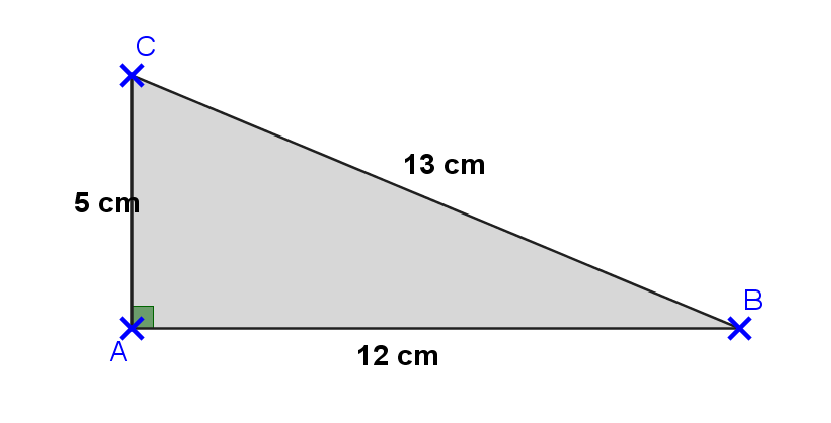
\includegraphics[scale=0.9]{aire2.eps} \\



Formule : . . . . . . . . . . . . . . .\\

Calculs : . . . . . . . . . . . . . . .\\

Réponse : . . . . . . . . . . . . . . .\\




\exo \\  Calculer l'aire du triangle EDF quelconque ci-dessous.\\

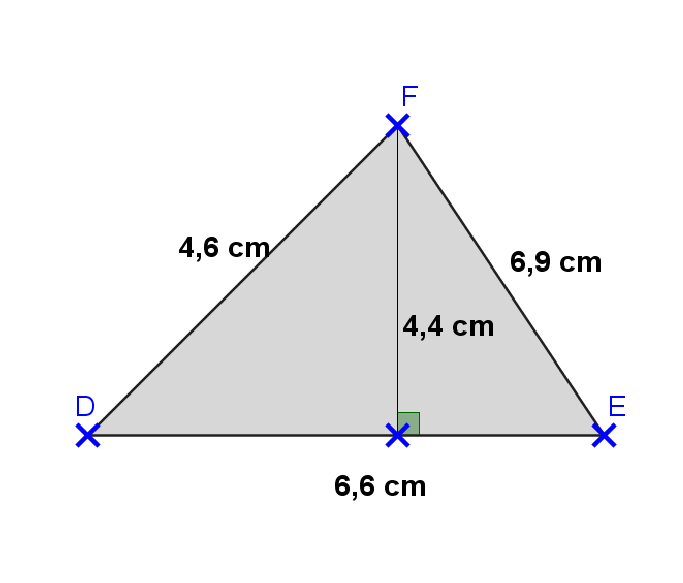
\includegraphics[scale=0.9]{aire3.eps} \\



Formule : . . . . . . . . . . . . . . .\\

Calculs : . . . . . . . . . . . . . . .\\

Réponse : . . . . . . . . . . . . . . .\\


\exo \\  Calculer l'aire du triangle JKL quelconque ci-dessous.\\

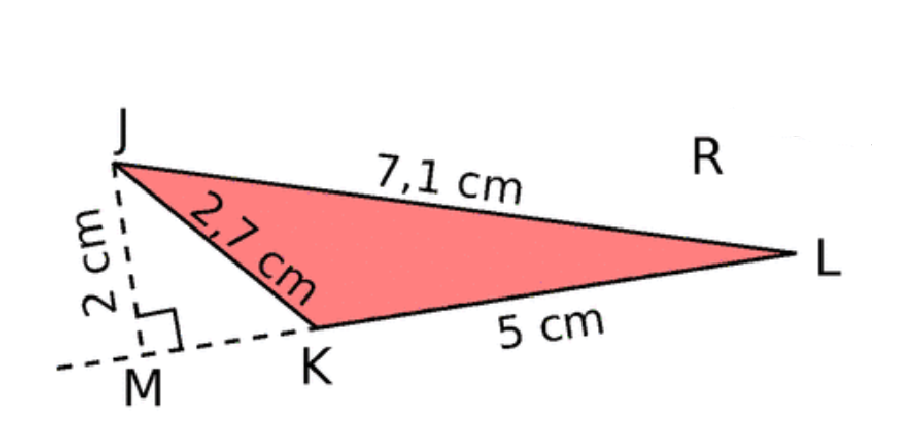
\includegraphics[scale=0.9]{aire4.eps} \\



Formule : . . . . . . . . . . . . . . .\\

Calculs : . . . . . . . . . . . . . . .\\

Réponse : . . . . . . . . . . . . . . .\\


\vspace*{1cm}

$\rightarrow$ \textbf{Aire de figures complexes}\\

\vspace*{0.5cm}


\exo \\ Calculer l'aire de la figure ci-dessous où IKLH est un rectangle.\\

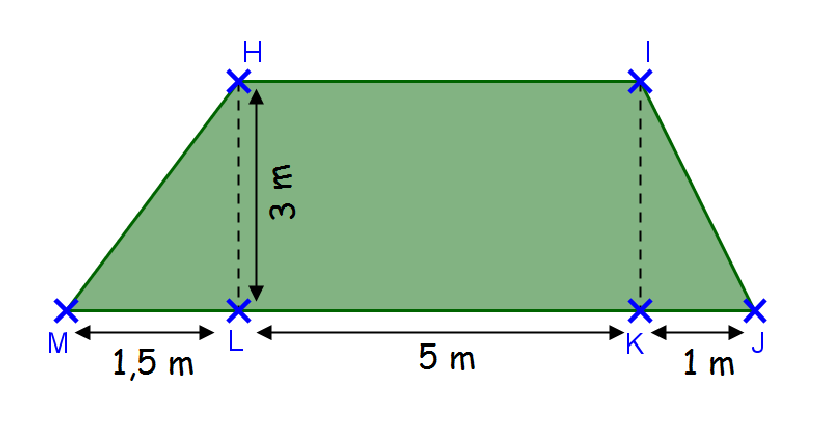
\includegraphics[scale=1]{airecomplexe10.eps} \\

Formules utilisées : . . . . . . . . . . . . . . .\\

Calculs :\\
\reponse[3]\\


Réponse : . . . . . . . . . . . . . . .\\



\exo \\ Calculer l'aire de la partie grisée suivante.\\

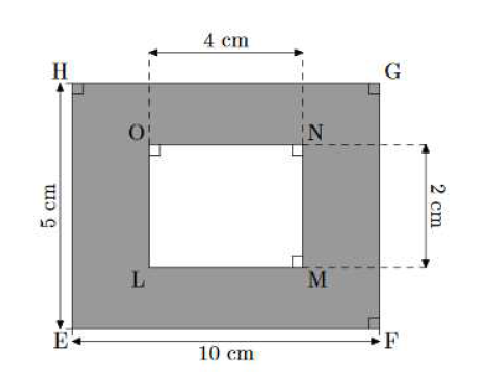
\includegraphics[scale=1]{airecomplexe5.eps} \\

Formules utilisées : . . . . . . . . . . . . . . .\\

Calculs :\\
\reponse[3]\\


Réponse : . . . . . . . . . . . . . . .\\



\exo \\ Calculer l'aire de la partie grisée suivante.\\

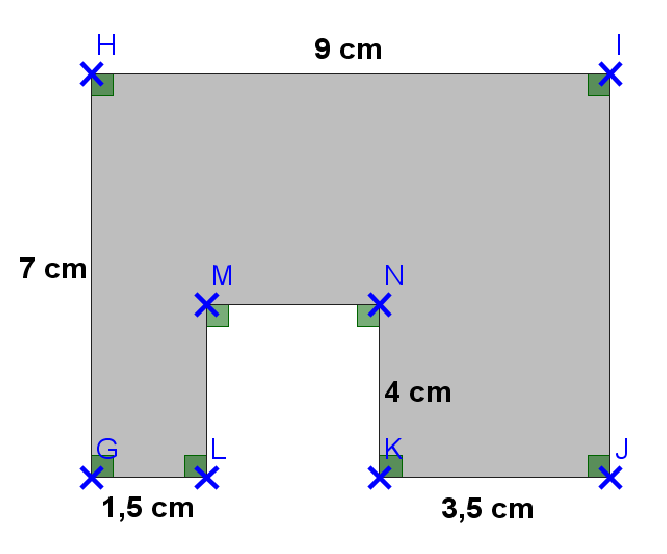
\includegraphics[scale=1]{airecomplexe6.eps} \\

Formules utilisées : . . . . . . . . . . . . . . .\\

Calculs :\\
\reponse[3]\\


Réponse : . . . . . . . . . . . . . . .\\







\begin{center}
{\Large \textbf{Niveau 4:}}
\end{center}

\vspace*{1cm}

$\rightarrow$ \textbf{Conversion des longueurs (m)}\\

\vspace*{0.5cm}





\exo \\ Exprimer les longueurs dans l'unité demandée.\\



\vspace{0.75cm}

\initqa \qa 7,4 dm = . . . . m\\

\qa 54,1 hm = . . . . m\\

\qa 78,2 mm = . . . . dm\\

\qa 3,51 km = . . . . cm\\

\qa 12,96 dam = . . . . mm\\

\qa 11,5 m = . . . . km\\



\exo \\ Voici quelques performances réalisées au championnat du monde d'athlétisme en 2003.\\

\begin{tabular}{|c|c|c|c|}
\hline 
Perche & Hauteur & Triple saut & Longueur \\ 
\hline 
0,0059 km & 235 cm & 177,2 dm & 0,832 dam \\ 
\hline 
\end{tabular} 

\vspace*{0.5cm}

Écrire ces performances en mètre.\\


\begin{tabular}{|c|c|c|c|}
\hline 
Perche & Hauteur & Triple saut & Longueur \\ 
\hline 
. . . . m & . . . . m & . . . . m & . . . . m \\ 
\hline 
\end{tabular} 


\vspace*{1cm}

$\rightarrow$ \textbf{Conversion : unités d'aire ($m^{2}$)}\\

\vspace*{0.5cm}


\exo \\ Compléter par les symboles $<$, $>$, $=$ :\\

\bmul{2}

\initqa \qa 16 $m^{2}$ . . . 0,2 $dam^{2}$ \\

\qa 43 $dm^{2}$ . . . 0,5 $m^{2}$ \\

\columnbreak

\qa 0,37 $dam^{2}$ . . . 380 $dm^{2}$\\

\qa 0,6 $hm^{2}$ . . . 5 000 $m^{2}$\\

\emul




\exo \\   Compléter les égalités suivantes.\\

\initqa \qa 2 $hm^{2}$ = . . . . . . . .  $m^{2}$\\

\qa 753 $cm^{2}$ = . . . . . . . .  $dm^{2}$\\

\qa . . . . .  $km^{2}$ = 71 000  $m^{2}$\\

\qa 5,36 . . . = 536  $m^{2}$\\

\qa 46 $m^{2}$ = . . . . . . . .  $cm^{2}$\\

\qa 6,41 $dm^{2}$ = . . . . . . . .  $mm^{2}$\\




\vspace*{1cm}

$\rightarrow$ \textbf{Périmètre d'un polygone / cercle}\\

\vspace*{0.5cm}


\exo \\ Calculer le périmètre du polygone ci-dessous.\\

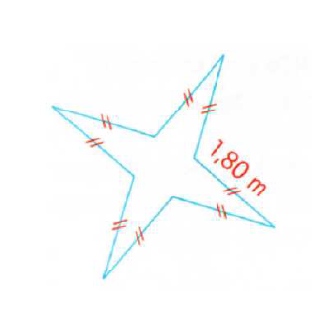
\includegraphics[scale=1]{perimetre11.eps} \\


Calculs : . . . . . . . . . . . . . . .\\

Réponse : . . . . . . . . . . . . . . .\\

\exo \\ Calculer le périmètre du polygone ci-dessous.\\

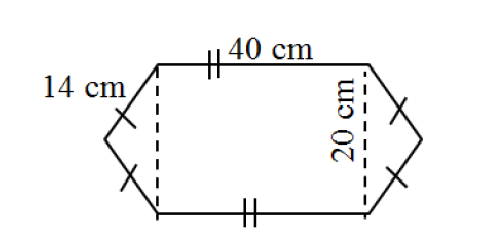
\includegraphics[scale=1]{perimetre12.eps} \\


Calculs : . . . . . . . . . . . . . . .\\

Réponse : . . . . . . . . . . . . . . .\\




\exo \\ Calculer le périmètre du polygone ci-dessous.\\

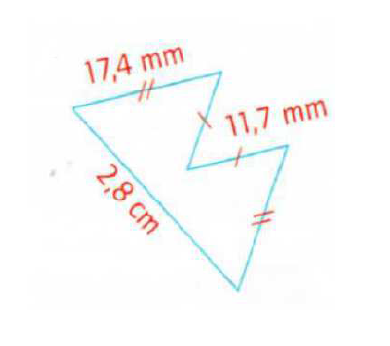
\includegraphics[scale=1]{perimetre9.eps} \\


Calculs : . . . . . . . . . . . . . . .\\

Réponse : . . . . . . . . . . . . . . .\\

\textbf{Indice : Pensez à convertir les longueurs dans la même unité avant de faire votre calcul.}\\




\exo \\ Calculer le périmètre du polygone ci-dessous.\\

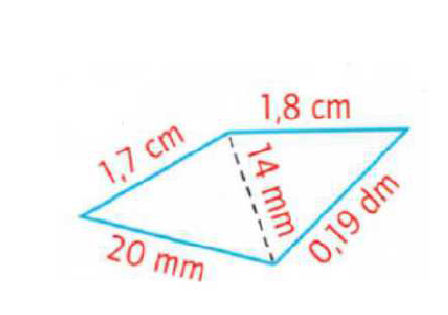
\includegraphics[scale=1]{perimetre10.eps} \\


Calculs : . . . . . . . . . . . . . . .\\

Réponse : . . . . . . . . . . . . . . .\\

\textbf{Indice : Pensez à convertir les longueurs dans la même unité avant de faire votre calcul.}\\



\exo \\ Compléter la formule pour calculer le périmètre d'un cercle de rayon \textit{r}.\\

$P=....................$\\



\exo \\ Compléter la formule pour calculer le périmètre d'un cercle de diamètre \textit{d}.\\

$P=....................$\\


\exo \\ Calculer le périmètre du cercle de centre A et de rayon  5 cm représenté ci-dessous.\\

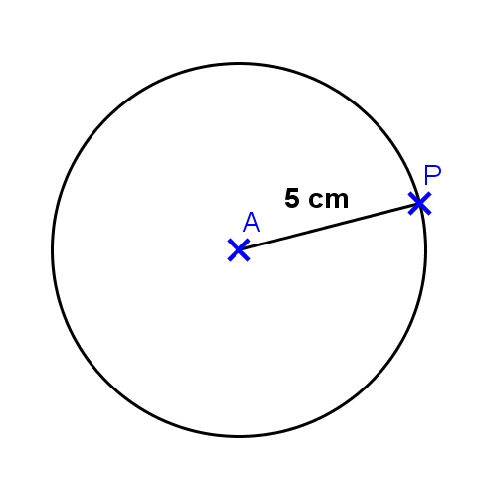
\includegraphics[scale=1]{perimetre13.eps} \\


Formule : . . . . . . . . . . . . . . .\\

Calculs : . . . . . . . . . . . . . . .\\

Réponse : . . . . . . . . . . . . . . .\\


\exo \\ Calculer le périmètre du cercle de centre O et de diamètre  100 dm représenté ci-dessous.\\

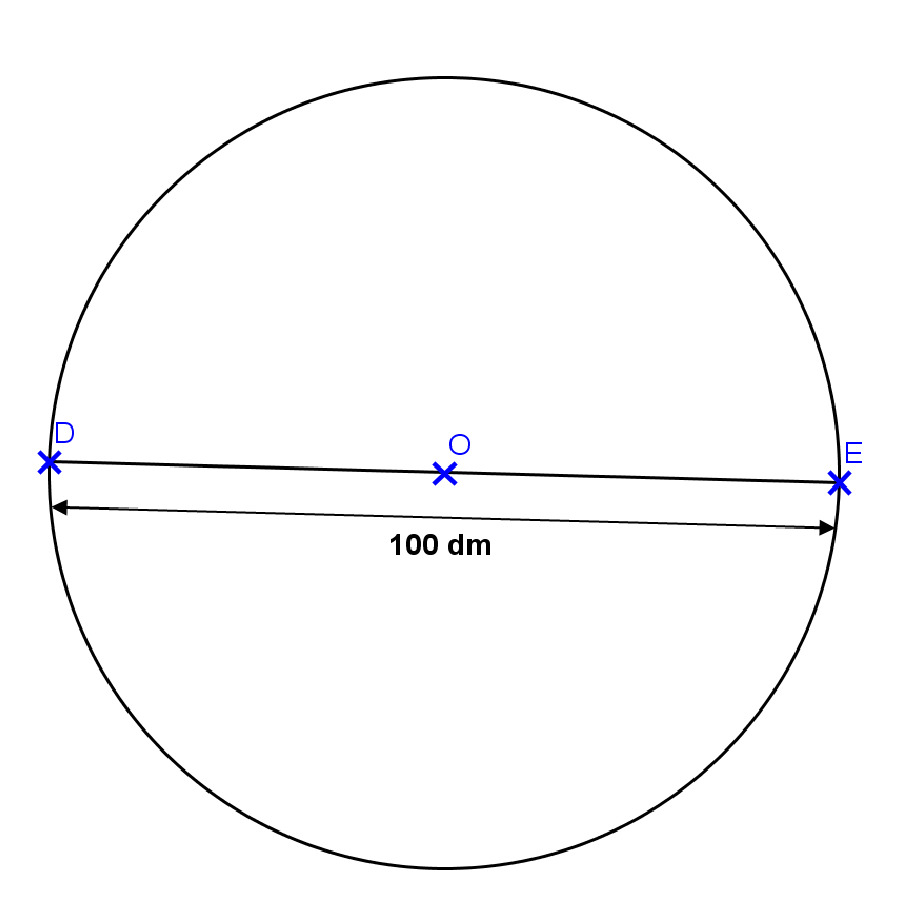
\includegraphics[scale=1]{perimetre14.eps} \\


Formule : . . . . . . . . . . . . . . .\\

Calculs : . . . . . . . . . . . . . . .\\

Réponse : . . . . . . . . . . . . . . .\\


\vspace*{1cm}

$\rightarrow$ \textbf{Périmètre de figures complexes}\\

\vspace*{0.5cm}



\exo \\ Calculer le périmètre de la figure ci-dessous, après avoir complété sa description.\\

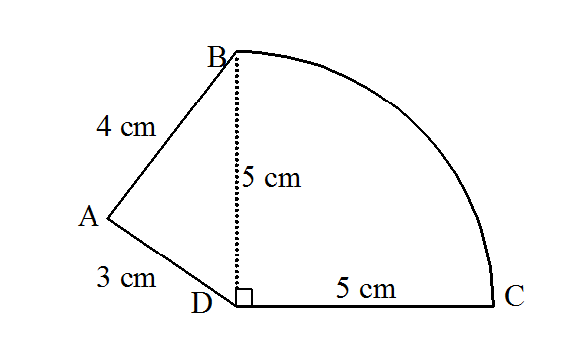
\includegraphics[scale=1]{complexe4.eps} 

\textbf{Description :} Cette figure est composée de . . .  quart(s) de cercle de même rayon et de . . . . segment(s).\\

Formule(s) utilisée(s) : . . . . . . . . . . . . . . .\\

Calculs :\\
\reponse[2]\\

Réponse : . . . . . . . . . . . . . . .\\




\exo \\ Calculer le périmètre de la figure ci-dessous, après avoir complété sa description.\\

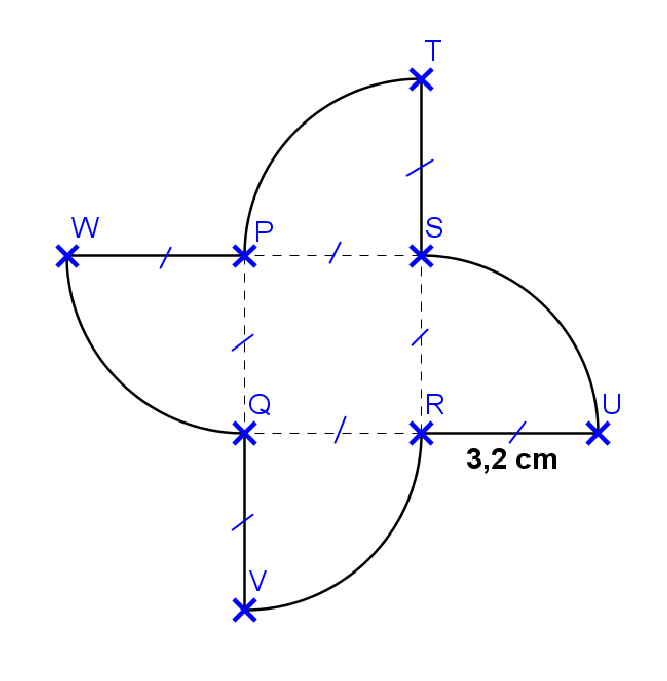
\includegraphics[scale=1]{complexe6.eps} 

\textbf{Description :} Cette figure est composée de . . .  quart(s) de cercle de même rayon et de . . . . segment(s).\\

Formule(s) utilisée(s) : . . . . . . . . . . . . . . .\\

Calculs :\\
\reponse[2]\\

Réponse : . . . . . . . . . . . . . . .\\






\vspace*{1cm}

$\rightarrow$ \textbf{Aire de figures usuelles}\\

\vspace*{0.5cm}

\exo \\ Calculer l'aire d'un rectangle de longueur 7 m et de largeur 0,4 dm.\\

Formule : . . . . . . . . . . . . . . .\\

Calculs :. . . . . . . . . . . . . . .\\

Réponse : . . . . . . . . . . . . . . .\\


\exo \\  Calculer l'aire du triangle DFE quelconque ci-dessous.\\

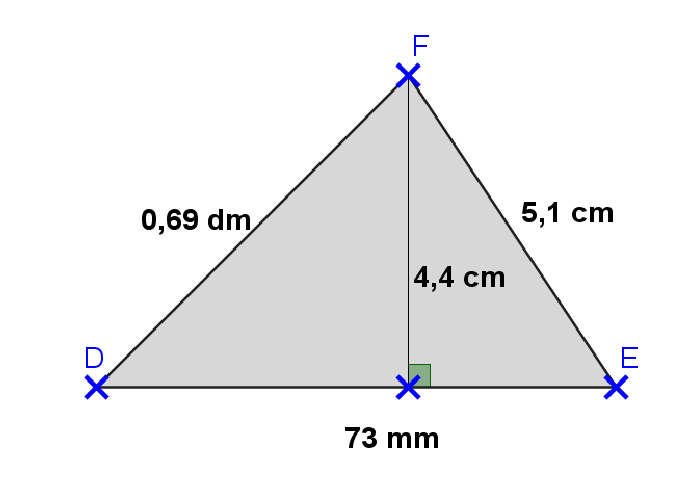
\includegraphics[scale=0.9]{aire5.eps} \\



Formule : . . . . . . . . . . . . . . .\\

Calculs : . . . . . . . . . . . . . . .\\

Réponse : . . . . . . . . . . . . . . .\\


\textbf{Indice : Pensez à convertir les longueurs avant de faire votre calcul.}\\


\exo \\ Compléter la formule pour calculer l'aire d'un disque de rayon \textit{r}.\\

$A=....................$\\



\exo \\ Calculer l'aire d'un disque de rayon 2 m.\\


Formule : . . . . . . . . . . . . . . .\\

Calculs : . . . . . . . . . . . . . . .\\

Réponse : . . . . . . . . . . . . . . .\\



\exo \\ Calculer l'aire du disque de centre O et de rayon 10 cm représenté ci-dessous.\\

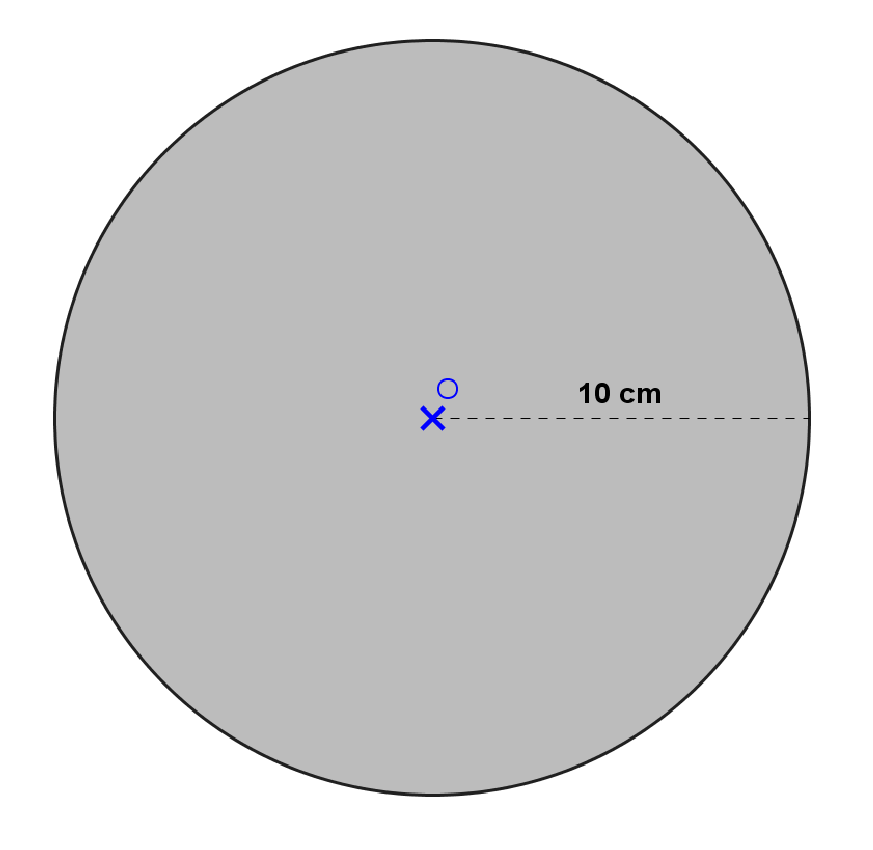
\includegraphics[scale=1]{aire6.eps} \\


Formule : . . . . . . . . . . . . . . .\\

Calculs : . . . . . . . . . . . . . . .\\

Réponse : . . . . . . . . . . . . . . .\\



\vspace*{1cm}

$\rightarrow$ \textbf{Aire de figures complexes}\\

\vspace*{0.5cm}


\exo \\ M. Dupont habite à Paris et vend un terrain représenté ci-dessous, au prix de 5 000 euros le $m^{2}$.\\

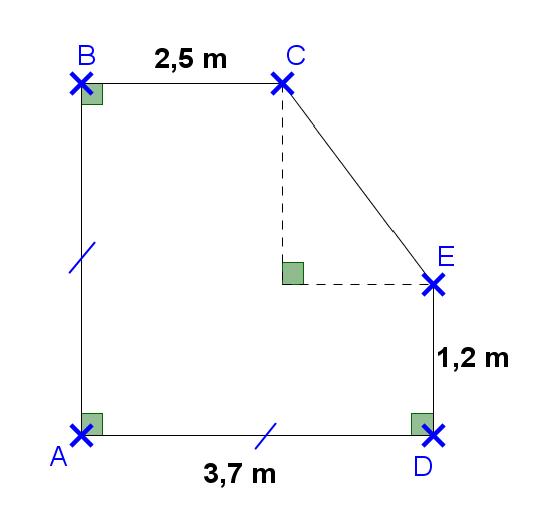
\includegraphics[scale=1]{airecomplexe1.eps} \\

Quel est le prix de ce terrain ?\\



Formules utilisées : . . . . . . . . . . . . . . .\\

Calculs :\\
\reponse[3]\\

Réponse : . . . . . . . . . . . . . . .\\




\exo \\ Calculer l'aire de la figure ci-dessous. Vous donnerez une valeur approchée par excès à l'unité près.\\

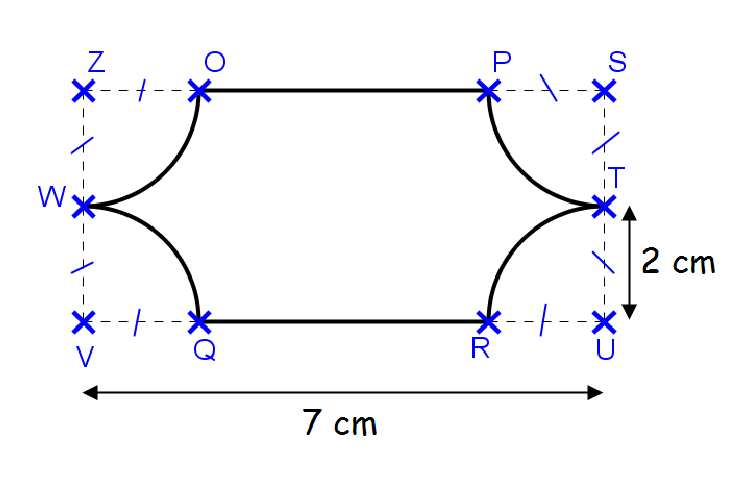
\includegraphics[scale=1]{airecomplexe7.eps} \\

Formules utilisées : . . . . . . . . . . . . . . .\\

Calculs :\\
\reponse[3]\\


Réponse : . . . . . . . . . . . . . . .\\





\exo \\ Calculer l'aire de la figure ci-dessous où ABCD est un rectangle. Vous donnerez une valeur approchée par excès à l'unité près.\\

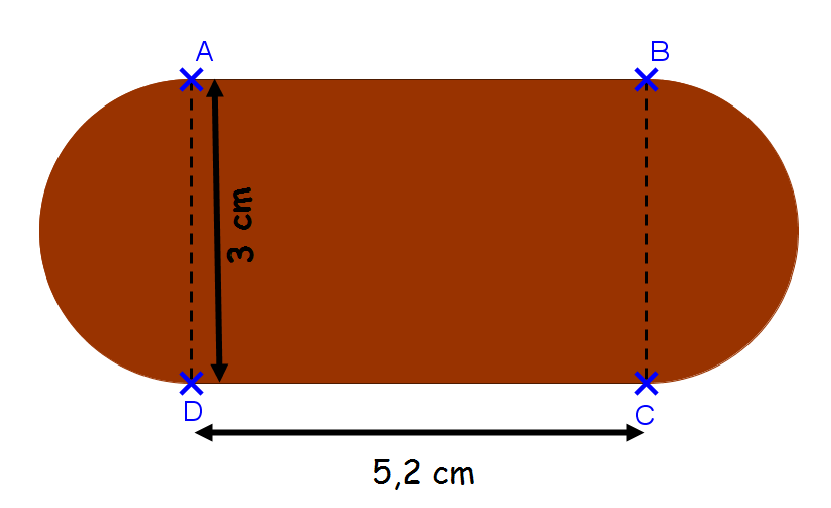
\includegraphics[scale=1]{airecomplexe8.eps} \\

Formules utilisées : . . . . . . . . . . . . . . .\\

Calculs :\\
\reponse[3]\\


Réponse : . . . . . . . . . . . . . . .\\









\begin{center}
{\Large \textbf{Niveau 5 :}}
\end{center}

\vspace*{1cm}

$\rightarrow$ \textbf{Conversion des longueurs (m)}\\

\vspace*{0.5cm}





\exo \\ Exprimer les longueurs dans l'unité demandée.\\


\bmul{2}
 5,6 m = . . . cm.\\


25,8 km = . . . m.\\


 328 dm = . . . dam.\\

\columnbreak

 7,85 m = 7850 ....   \\

9 dm = 0,009 ....\\

 4,036 dam = 40 360 . . .\\

\emul


\exo \\ Ranger ces objets du plus court au plus long.\\

Stylo : 12,57 cm \hspace*{1cm} Crayon : 126 mm\\

Ciseaux : 0,21 m \hspace*{1cm} Feutre : 12,5 cm\\

\noindent \reponse[3]\\


\exo \\ Compléter par les symboles $<$, $>$, $=$ :\\

\bmul{2}

\initqa \qa 0,49 km . . . 490 000 mm \\

\qa 22,3 km . . . 3 220 m \\

\columnbreak

\qa 2,78 m . . . 2 870 mm\\

\qa 11,32 m . . . 1 123 cm\\

\emul


\vspace*{1cm}

$\rightarrow$ \textbf{Conversion : unités d'aire ($m^{2}$)}\\

\vspace*{0.5cm}



\exo \\ Ranger ces aires par ordre croissant.\\

750 $cm^{2}$ \hspace*{1.5cm} 0,21 $m^{2}$ \hspace*{1.5cm} 63,8 $dm^{2}$ \hspace*{1.5cm} 0,0035 $dam^{2}$ \\

\noindent \reponse[2]\\

\exo \\ Caroline souhaite vendre son terrain de 1,5 ha. Sur le marché, le mètre carré vaut 4 euros.\\

Quel est le prix de vente de ce terrain ?\\

Calcul :\\
\reponse[2]\\


Réponse :\\
\reponse[1]\\


\vspace*{1cm}

$\rightarrow$ \textbf{Périmètre d'un polygone / cercle}\\

\vspace*{0.5cm}



\exo \\ Calculer le périmètre des 3 figures suivantes (arrondir au cm pour le cercle) puis en déduire quelle figure a le plus grand périmètre.\\


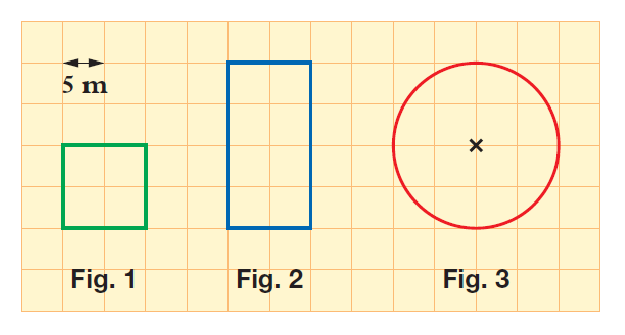
\includegraphics[scale=1]{perimetre15.eps} \\


Formules : . . . . . . . . . . . . . . . et  . . . . . . . . . . . . . . . et . . . . . . . . . . . . . . .\\

Calculs : . . . . . . . . . . . . . . .\\

Réponse : . . . . . . . . . . . . . . .\\



\exo \\ Calculer le périmètre d'un cercle de 3,5 cm de rayon.\\

Formule : . . . . . . . . . . . . . . . \\

Calculs : . . . . . . . . . . . . . . .\\

Réponse : . . . . . . . . . . . . . . .\\



\exo \\  Calculer la circonférence d'un cercle de diamètre 10 m.\\


Formule : . . . . . . . . . . . . . . . \\

Calculs : . . . . . . . . . . . . . . .\\

Réponse : . . . . . . . . . . . . . . .\\



\exo \\ Calculer le périmètre d'un demi-cercle de centre O et de rayon 5 cm représenté ci-dessous.\\

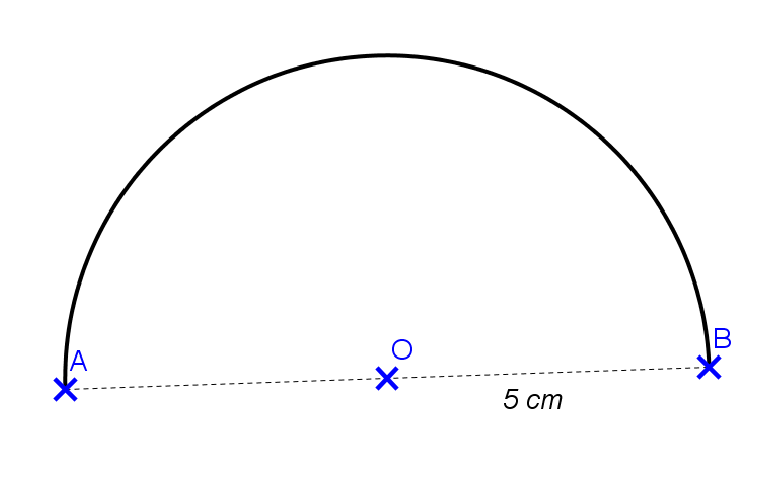
\includegraphics[scale=1]{perimetre16.eps} \\

Formule utilisée : . . . . . . . . . . . . . . . \\

Calculs : . . . . . . . . . . . . . . .\\

Réponse : . . . . . . . . . . . . . . .\\

\exo \\ Calculer le périmètre d'un quart-cercle de centre F et de rayon 3,5 dm représenté ci-dessous.\\

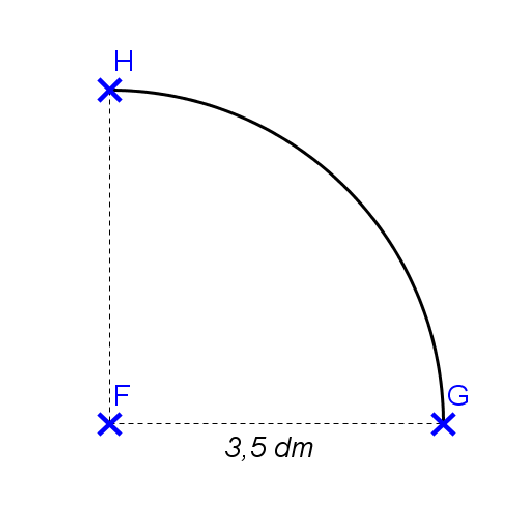
\includegraphics[scale=1]{perimetre17.eps} \\

Formule utilisée : . . . . . . . . . . . . . . . \\

Calculs : . . . . . . . . . . . . . . .\\

Réponse : . . . . . . . . . . . . . . .\\

\exo \\ Calculer le périmètre des trois quarts-cercle de centre O et de rayon 3 cm représenté ci-dessous.\\

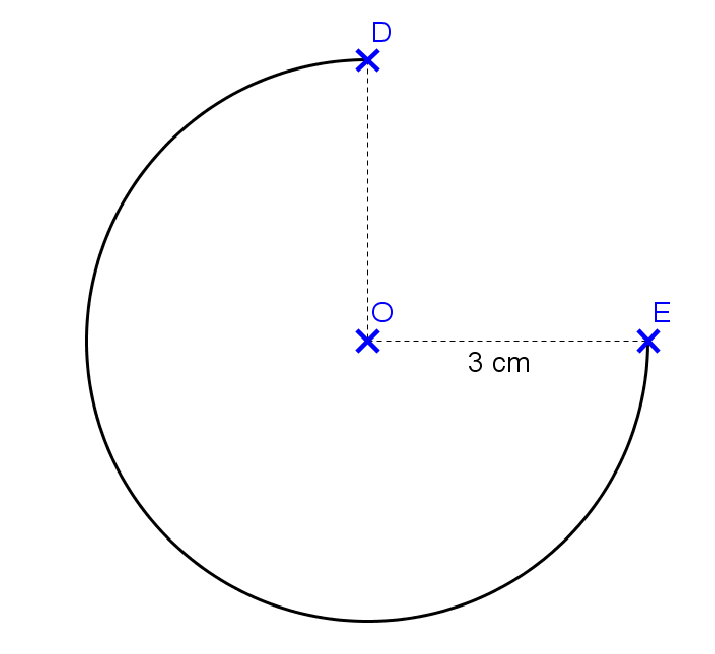
\includegraphics[scale=1]{perimetre18.eps} \\

Formule utilisée : . . . . . . . . . . . . . . . \\

Calculs : . . . . . . . . . . . . . . .\\

Réponse : . . . . . . . . . . . . . . .\\

\vspace*{1cm}

$\rightarrow$ \textbf{Périmètre de figures complexes}\\

\vspace*{0.5cm}




\exo \\ Calculer le périmètre de la figure ci-dessous, après avoir complété sa description.\\

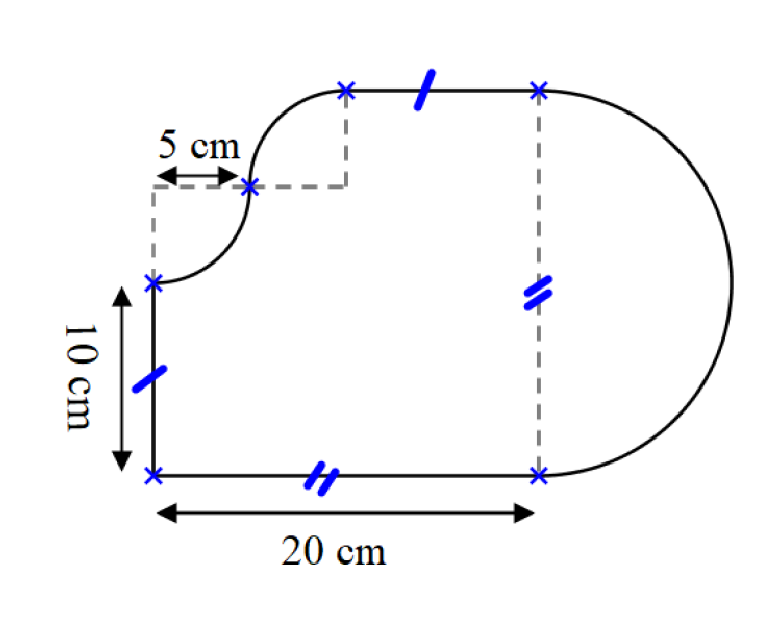
\includegraphics[scale=0.8]{complexe5.eps} \\

\textbf{Description :} Cette figure est composée de . . .  quart(s)cercle de même rayon, de . . . demi-cercle de même rayon et  de . . . . segment(s).\\

Formule(s) utilisée(s) : . . . . . . . . . . . . . . .\\

Calculs :\\
\reponse[2]\\

Réponse : . . . . . . . . . . . . . . .\\



\exo \\ Calculer le périmètre de la figure ci-dessous, après avoir complété sa description.\\

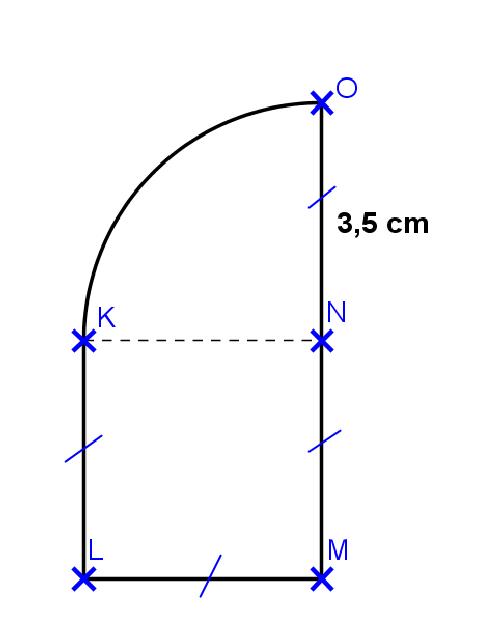
\includegraphics[scale=1]{complexe7.eps} 

\textbf{Description :} Cette figure est composée de . . .  quart(s) de cercle de même rayon et de . . . . segment(s).\\

Formule(s) utilisée(s) : . . . . . . . . . . . . . . .\\

Calculs :\\
\reponse[2]\\

Réponse : . . . . . . . . . . . . . . .\\



\vspace*{1cm}

$\rightarrow$ \textbf{Aire de figures usuelles}\\

\vspace*{0.5cm}




\exo \\ Calculer l'aire d'un disque de diamètre 8 m.\\


Formule : . . . . . . . . . . . . . . .\\

Calculs : . . . . . . . . . . . . . . .\\

Réponse : . . . . . . . . . . . . . . .\\



\exo \\ Calculer l'aire du disque de centre C et de diamètre 20 mm représenté ci-dessous.\\

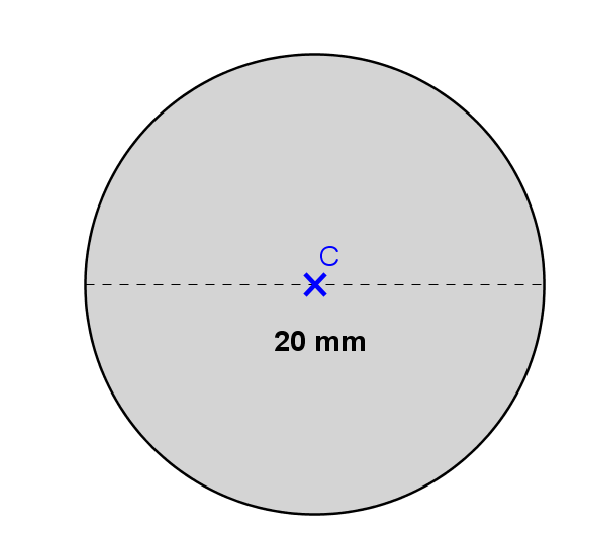
\includegraphics[scale=1]{aire7.eps} \\


Formule : . . . . . . . . . . . . . . .\\

Calculs : . . . . . . . . . . . . . . .\\

Réponse : . . . . . . . . . . . . . . .\\


\exo \\ Calculer l'aire du demi-disque ci-dessous.\\

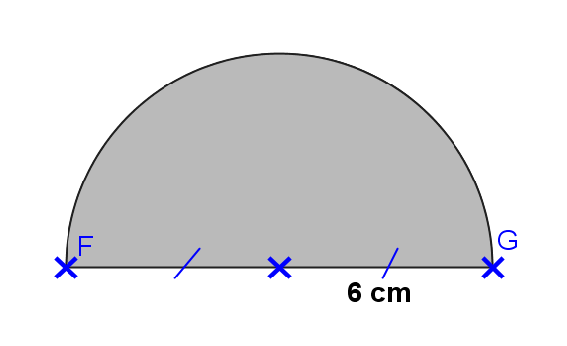
\includegraphics[scale=1]{aire8.eps} \\


Formule : . . . . . . . . . . . . . . .\\

Calculs : . . . . . . . . . . . . . . .\\

Réponse : . . . . . . . . . . . . . . .\\



\exo \\ Calculer l'aire du quart de disque ci-dessous.\\

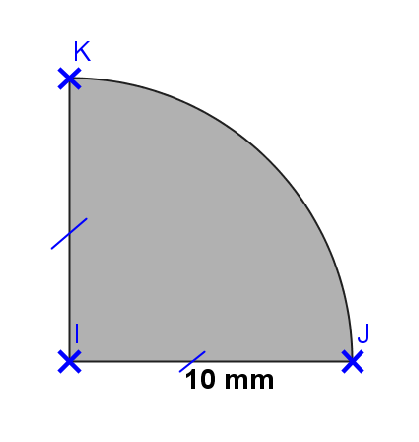
\includegraphics[scale=1]{aire9.eps} \\


Formule : . . . . . . . . . . . . . . .\\

Calculs : . . . . . . . . . . . . . . .\\

Réponse : . . . . . . . . . . . . . . .\\


exo \\ Calculer l'aire des trois quart de disque ci-dessous.\\

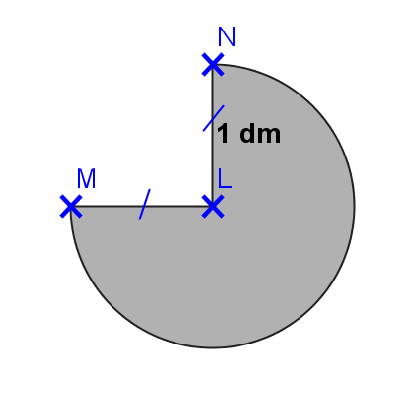
\includegraphics[scale=1]{aire10.eps} \\


Formule : . . . . . . . . . . . . . . .\\

Calculs : . . . . . . . . . . . . . . .\\

Réponse : . . . . . . . . . . . . . . .\\


\vspace*{1cm}

$\rightarrow$ \textbf{Aire de figures complexes}\\

\vspace*{0.5cm}



\exo \\ Dans un jardin public, on souhaite semer du gazon autour d'un bassin d'eau. Sur le schéma ci-dessous le disque de centre E représente le bassin d'eau. Tout le reste représente la future pelouse.\\

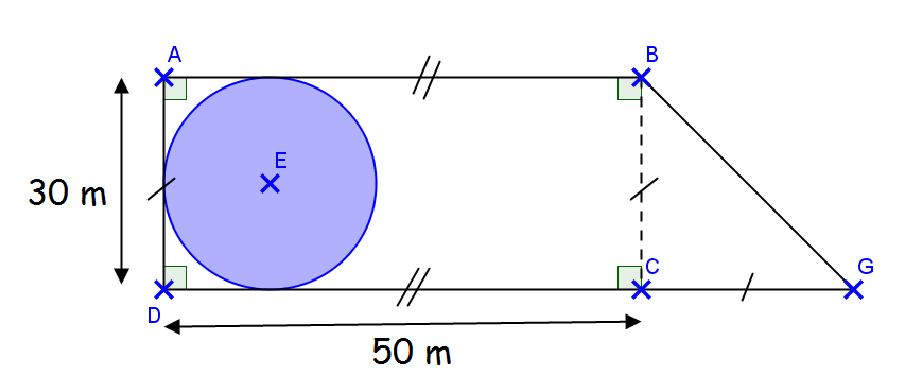
\includegraphics[scale=1]{airecomplexe3.eps} \\


Quelle est l'aire de la future pelouse ?\\

Formules utilisées : . . . . . . . . . . . . . . .\\

Calculs :\\
\reponse[3]\\


Réponse : . . . . . . . . . . . . . . .\\



\exo \\ Calculer l'aire de la figure orange ci-dessous. Vous donnerez une valeur approchée par excès au dixième près.\\

\includegraphics[scale=1]{airecomplexe9.eps} \\

Formules utilisées : . . . . . . . . . . . . . . .\\

Calculs :\\
\reponse[3]\\


Réponse : . . . . . . . . . . . . . . .\\


\end{document}
